\section*{3-$\gamma$ Decay Monte Carlo Simulation}

Measured 3-$\gamma$ from o-Ps decay, count only a fraction of the whole 3-$\gamma$ decay yield. This is due to the fact that the triple coincidence in the setup is only between detectors at 120$^\circ$. In order to get a correct estimate of the total 3-$\gamma$ events generated by o-Ps decay a Monte Carlo Simulation was used. The aim of the simulation is to numerically estimate the ratio:
\begin{equation*}
 f_{3-\gamma}^{Geom.} = \dfrac{\#\text{3-}\gamma\text{ events at 120}^\circ}{\#\text{total 3-}\gamma \text{ events}}
\end{equation*}

The simulation code\footnote{\noindent The code is available at:\\ \href{https://github.com/LucaMors/Physics_Lab_Reports/tree/master/Positronium/Analysis/Simulation}{github.com/LucaMors/Physics\_Lab\_Reports/tree/master/Positronium/Analysis/Simulation}} is built by three main part:
\begin{enumerate}
\item Event Generator
\item Experimental Setup
\item Run Manager
\end{enumerate}

\subsection*{Event Generator}

The event generator handle the photon creation from o-Ps decay. The algorithm used for an event generation is the following:
\begin{algorithm}
\caption{o-Ps Decay Photon Generator}\label{euclid}
\begin{algorithmic}[1]
\State Sample the theoretical energy distribution of photon from o-Ps decay, obtaining the energy of the first $\gamma$.
\State Sample a random point on a sphere surface for the purpose of obtaining the direction for momentum versor.
\State Scale momentum vector according to the sampled energy.
\State Repeat 1-3 for the 2$^{nd}\ \gamma$.
\State By imposing momentum conservation obtain the 3$^{nd}\ \gamma$ momentum vector.
\State From previously obtained vector get 3$^{nd}\ \gamma$ energy.
\State Sum the energy of all of the three $\gamma$ and check if energy conservation holds. If yes return the three Photon object otherwise return to 1.
\end{algorithmic}
\end{algorithm}

The theoretical energy distribution used to sample the photons energy is reported in \cite{ore1949three}.

\subsection*{Experimental Setup}

This part of code handle detector creation and positioning. A detector object is defined by a position vector $\vec{P_d}$ and by a edge vector $\vec{P}_{\text{edge}}$ that point to point belong to detector face edge and is completely determined by the detector face radius (we are considering cylindrical detectors). In order to check if an emitted $\gamma$ impinges onto a detector the code check if the angle ($\alpha_\gamma$) between $\vec{P}_d$ and $P_\gamma$ ($\gamma$-ray momentum) is lower than the half-aperture ($\varphi$) of the cone defined by our detector ( that is the angle between $\vec{P}_d$ and the edge vector $\vec{P}_{\text{edge}}$) as sketched Fig. \ref{Fig: angle det check}.

\begin{figure}[H]
\centering
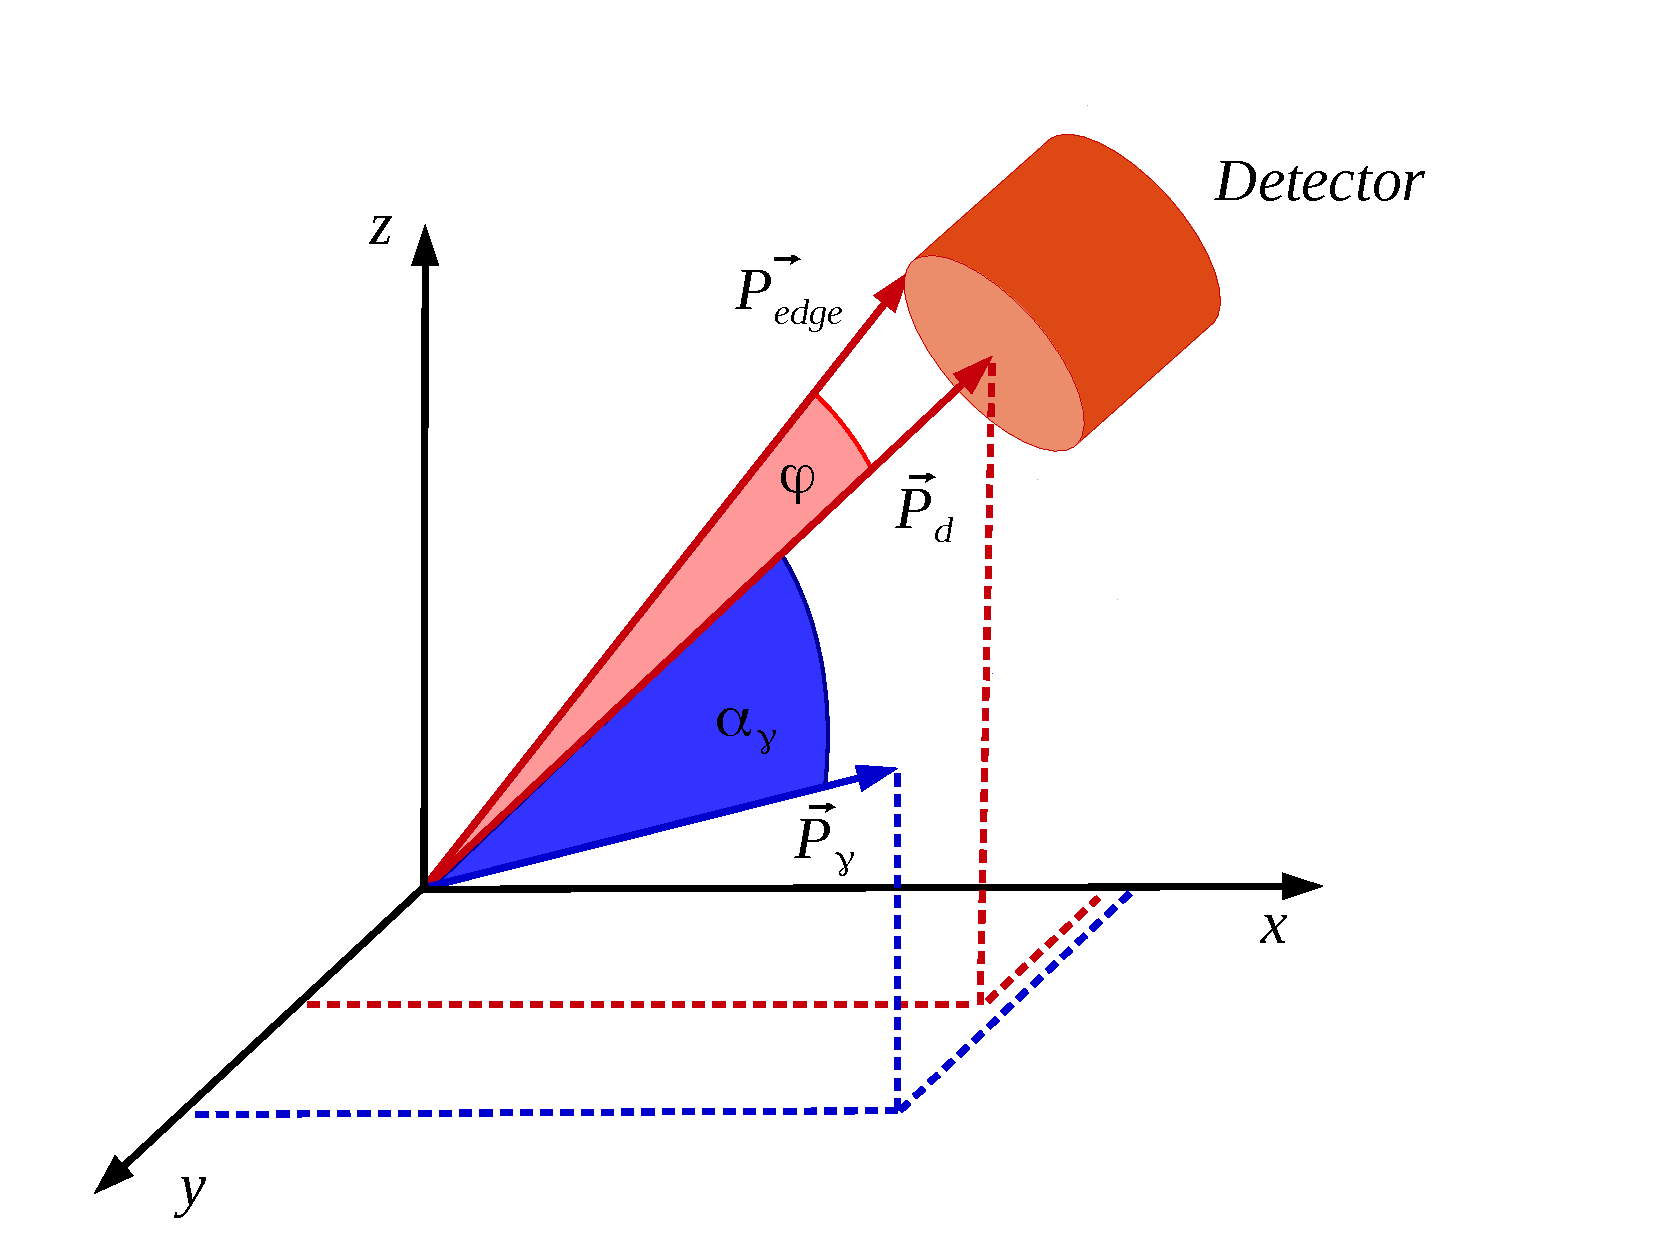
\includegraphics[width = 0.7\textwidth]{check_detector}
\caption{Detector and $\gamma$ angle notation. The situation presented in this figure is that of a rejected gamma.}
\label{Fig: angle det check}
\end{figure}


\subsection*{Run Manager}

This last part of the code handle the coincidence between detectors and the extraction of the required information.

Using the implemented code a simulation of $10^7$ events was performed and the resulting plots are presented in Fig. \ref{Fig: simulation result}.

\begin{figure}[H]
\centering
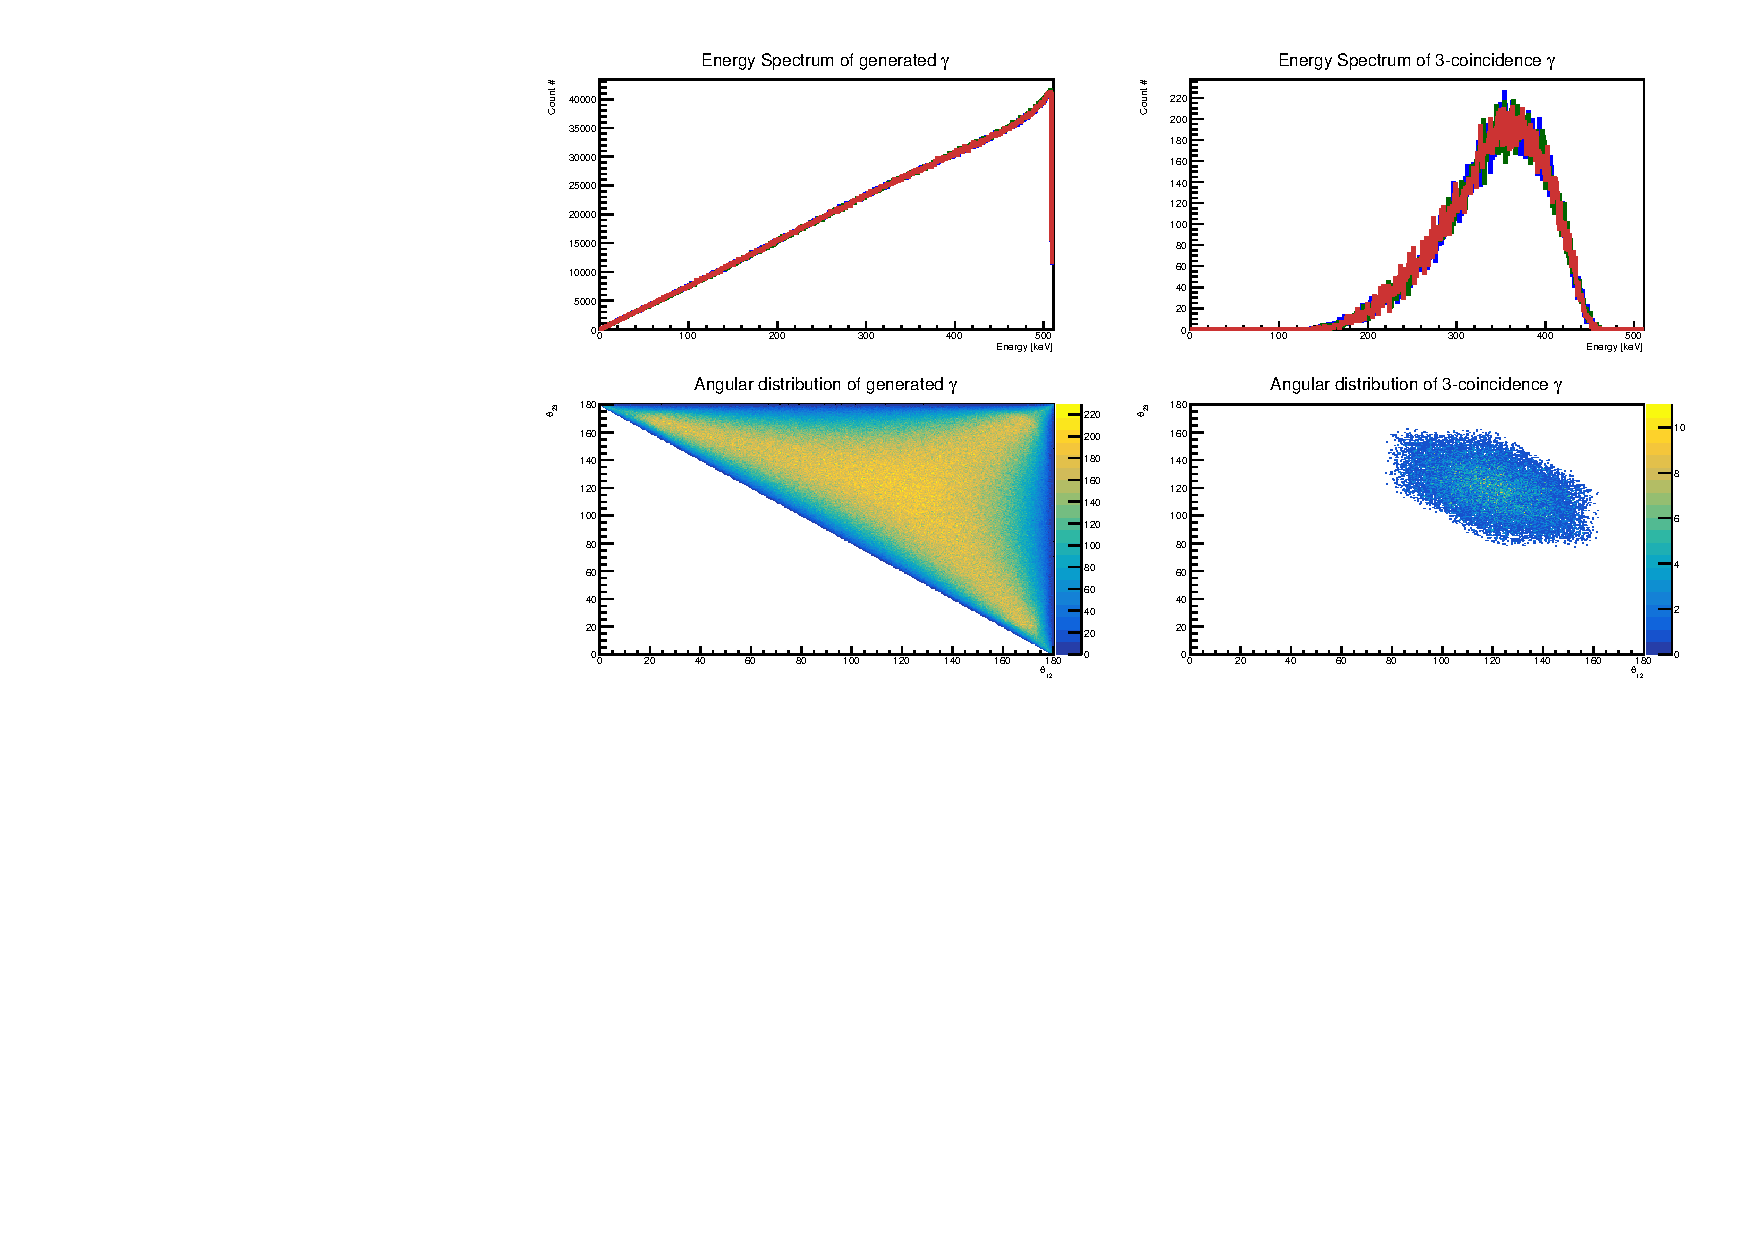
\includegraphics[width = \textwidth]{result}
\caption{(a) Theoretical Energy distribution of generated gamma. (b) Energy spectrum of the 3-coincident $\gamma$ events. (c) Angular distribution of generated events. (d) Angular distribution of 3-coincident $\gamma$ events.}
\label{Fig: simulation result}
\end{figure}

The simulation founds 
